\chapter{The Implementation of GIMMIX}

Now that the entire MMIX architecture has been explained, the simulator GIMMIX should be described. As already mentioned in the introduction, GIMMIX has been developed with the goal to be able to port an operating system to it. Therefore GIMMIX pursues to be correct (which implies to be not more complex than necessary), implement MMIX completely and offer a convenient and productive user interface, so that an OS can be debugged.

This chapter splits the depiction of GIMMIX into five parts. At first, the design decisions for the implementation are explained, followed by an overview of the simulator. Subsequently, the implementation of the MMIX architecture (the "core") is described in detail and yet existing devices are introduced shortly. Finally, the command line interface (CLI), which allows it to debug an OS or arbitrary other programs for MMIX, is presented.

\section{Basic Design Decisions}

Before starting with the description of the simulator, a few general design decisions that have been made should be explained.

\subsection{No Pipelining}

At first, it has been decided to abandon \glslink{Pipelining}{pipelining}. Since it is a simulator, \ie implemented in software, and has not the goal to explore the difficulties for a potential hardware \glslink{Pipelining}{pipelining} implementation or similar, using \glslink{Pipelining}{pipelining} would not bring advantages. Without it, the simulator is much simpler and thus the correctness is easier to achieve.

\subsection{Uninterruptible Instructions}

Similarly to the previous one and a bit related to it, it has been decided to make instructions uninterruptible, \ie an instruction is either executed completely or not at all, as far as no \glslink{Exception}{program or machine exception} occurs. As mentioned in \ref{sec:mmix-interruptibility} of chapter \ref{ch:mmix-arch}, MMIX allows it to make complex instructions like \mi{POP} or \mi{SAVE} interruptible by encoding the current state of computation in \sr{XX}, \sr{YY} and \sr{ZZ}. But it does not require implementations to do that, which means that it is specification conform to make all instructions uninterruptible. \citep[pg. 27]{mmix-doc}

Without this decision, GIMMIX would have required a concept that allows it to execute instructions in multiple steps, pause them for \glslink{Interrupt}{interrupts} and resume them later. This would have made it a lot more complex, without leading to real advantages for similar reasons as in the previous decision. Thus, for simplicity all instructions in GIMMIX are uninterruptible.

\subsection{Programming Language}

Obviously, when one wants to run an operating system in a simulator, \ie a program that implements the whole simulated machine in software, efficiency is very important. Additionally, a lot of control over the produced machine code is necessary to be able to imitate the exact behaviour of the simulated machine. Therefore it has been decided to use the programming language C, which both allows to build efficient programs and offers a lot of control. Additionally, MMIX-SIM and MMIX-PIPE are implemented in C as well\footnote{As mentioned, they are written with CWEB, which produces C code in the end.}, so that it is easier to use code from them, such as the floating point algorithms.

Since an octa is the word quantity of MMIX, it will be used at nearly all places in the simulator. Therefore, its representation affects more or less the whole code. Using \glslink{C89C99}{C89} on a 32-bit platform would mean, that no 64-bit type is available \citep{llgccext}. Thus, a struct would have to be created, that contains two 32-bit integers; one for the upper half of the octa and one for the lower half. Of course, every operation that is done with an octa, would have to be broken down to operations with the two 32-bit integers. In other words, the whole code of the simulator would get a lot more difficult to read and write, just because of the fact that there is no 64-bit type.

But there is an alternative. \glslink{C89C99}{C99} provides the so called \i{exact-width integer type} `uint64_t`, which does always correspond to an unsigned 64-bit integer, independent of the underlying platform \citep{uint64t}. That is, the compiler will arrange things, such that this type (including all possible operations with it) is available. Although most currently available compilers offer no complete implementation of \glslink{C89C99}{C99} yet \citep{c99supp}, even the old version 3.0 (released 2001 \citep{gccrel}) of the GNU C Compiler, which is used in this project, supports this feature including many other useful ones \citep{gcc30c99}. For these reasons, \glslink{C89C99}{C99} has been selected, but GIMMIX will only utilize some basic features of it such as exact-width integer types, "`//` comments", mixed declarations and code, initialization in for-loops and `snprintf`, which are available in \gls{gcc} and should be in almost all other compilers as well.

\subsection{Host Platform}

The host platform, \ie the platform that runs the simulator, is expected to be a Linux system. Although most parts of GIMMIX are platform independent, some of them -- like the simulated terminals for example -- assume Linux. Furthermore, the simulator core (excluding \eg some test generation programs, that expect x86) uses only standard \glslink{C89C99}{C99}, which means it should be hardware independent (but it has not been tested with different hardware).

Since both 32 and 64-bit platforms are widely spread nowadays, GIMMIX has the effort to support both of them. This is mostly achieved behind the scenes by adding a layer on top of the `printf`, `scanf` and `strtol` families. For the first two families, the layer lets the user specify the size of an argument with 'O','T','W' or 'B' (additionally to 'h', 'l' and 'L') for octa, tetra, wyde or byte, respectively. For `strtol`, the layer calls simply either `strtol` or `strtoll`, depending on the platform. But there are a few other things to take care of. For example, when using logical or arithmetical negation, the result depends on the size of the operand. That means, \eg `-sizeof(octa)` could lead to different results. If the type of `sizeof(octa)` is 32 bit wyde, the logical negation would produce \haddrt{FFFF}{FFF8}, instead of the perhaps intended \haddro{FFFF}{FFFF}{FFFF}{FFF8}. Thus, whenever such operators are used with this intention, the operand has to be casted to an octa first.


\section{Overview}

Before explaining the main parts of GIMMIX, this section gives an overview and introduces the basic components, that are used throughout the code.

Conceptually, GIMMIX consists of several \i{modules} that interact with each other. The name of a module corresponds to a source file or folder in the directory \file{src} and to the associated header file or folder in the directory \file{include}. The following \gls{FMC} diagram illustrates the most important modules and their relationships, whereas the CLI, the core and the devices are only shown as black boxes for now:
\begin{figure}[H]
	\centering
	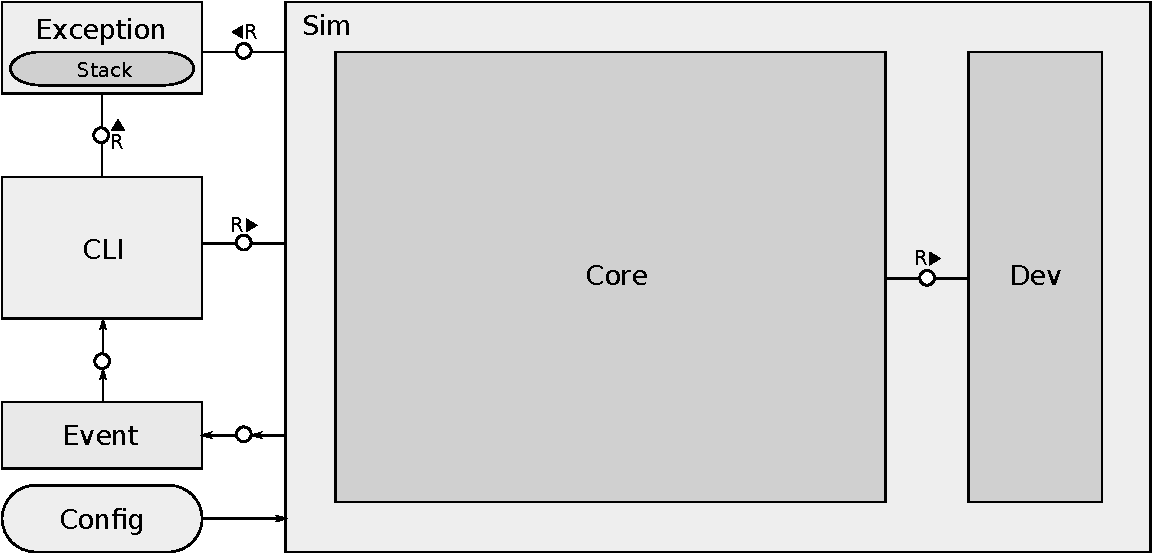
\includegraphics[width=\textwidth]{img/sim-fmc-crop.pdf}
	\caption{Architecture of GIMMIX in \protect\gls{FMC} notation}
	\label{fig:gimmix-arch}
\end{figure}
\noindent That means, the modules \i{core} and \i{dev}, to which the core sends requests for tasks like reading an octa from a specific physical address, are in a sense enveloped in \i{sim}. Sim supports some basic operations like initializing the whole system, resetting it or shutting it down. This is controlled by the module \i{CLI} (when running in interactive mode). The following sections describe the other general modules in the figure.

\subsection{Exception}

Although \glslink{Exception}{exception} handling in C via `setjmp` and `longjmp` is not as convenient and powerful as for example in Java, it offers some advantages. That is, it separates "normal" code from exceptional code and provides the possibility to handle an \glslink{Exception}{exception} only at places, where it can be handled in a sensible way. To achieve that and allow nested "try and catches", the module \i{exception} manages a stack of `jmp_buf`s, which hold the state created by `setjmp`. It is used for trips and traps in the core and also for \glslink{Exception}{exceptions} in the CLI. The most important functions are:
\begin{itemize}
	\item `ex_push(jmp_buf *environment)`:\\
	This function pushes the given environment onto the stack and is thus the equivalent to a `try`. The environment \i{has to} be created by the caller, because one can not jump back to a stack frame, that has been already destroyed.
	\item `ex_throw(int exception,octa bits)`:\\
	As the name suggests, it throws the \glslink{Exception}{exception} with given number and additional information in `bits`, which is used for example to specify what trip or trap should be triggered. That is, it calls `longjmp` with the topmost `jmpbuf` and `exception` as arguments, so that the caller of `setjmp` receives `exception` as return-value.
	\item `ex_pop()`:\\
	This function removes the topmost environment from the stack. Hence, it is the equivalent to the end of a try-catch-construct.
\end{itemize}
In this thesis, the term "\glslink{Exception}{exception}" without the prefix "arithmetical", "program" or "machine", refers to this concept, instead of the different \glslink{Exception}{exceptions} of MMIX.

\subsection{Event}

As already mentioned, GIMMIX offers a sophisticated CLI that should allow it to debug an operating system or other programs in a convenient way. To do so, the CLI needs of course access to the core, \ie it has to read the current state and should also be able to display the effect of an instruction or set breakpoints. Integrating all those facilities into the core would mean, that it gets more difficult to read and understand and it would also introduce strong coupling between the CLI and the core. Since the core is quite stable (the architecture is not expected to change much), but it may indeed be imaginable to provide a graphical user interface (GUI) to GIMMIX some day, it has been decided to work with events to supply the user interface with information. This way, the core is completely independent of the CLI and thus, assuming that a GUI is ready, it could replace the CLI within minutes, without affecting the core.

The module \i{event} implements this idea by providing `ev_register` to register a callback function for a specific event and `ev_unregister` to unregister it again. Additionally, events can be fired by calling `ev_fire`, `ev_fire1` or `ev_fire2` to raise an event with 0, 1 or 2 arguments, respectively. As figure \ref{fig:gimmix-arch} suggests, the core fires events and the event module forwards them to the CLI (and any other interested modules), which has registered the corresponding callbacks at the beginning. It is noteworthy, that if GIMMIX is used in non-interactive mode, the CLI will not be used at all and thus no callback will be registered, which will allow GIMMIX to be as performant as possible.

\subsection{Config}

Of course, GIMMIX should be configurable to some extent, which is realized by the module \i{config}. It consists of two categories of settings: the settings in the first one are configurable during compile time (\ie constants are used) and the other ones are configurable during runtime. The latter can be passed to GIMMIX as command line arguments. In a sense, the compile time options are those that would be fixed when GIMMIX were a solid piece of hardware (number of local registers, cache size, device addresses, \dots), while the runtime options could be changed more easily (amount of main memory, number of terminals, disk image, \dots). But of course, there are also practical reasons, why one has to be able to specify the disk image or the rom image via command line argument.


\section{Simulator Core}

This section describes the most important part of the simulator, \ie the implementation of the MMIX architecture.

\subsection{Structure}

The following figure breaks the core, that has been displayed as a black box in the previous \gls{FMC} diagram, further down into pieces:
\begin{figure}[H]
	\centering
	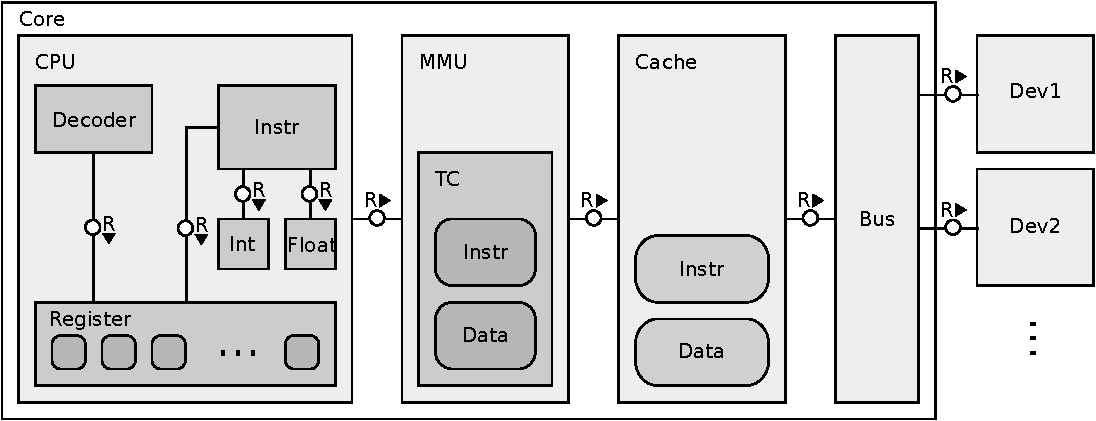
\includegraphics[width=\textwidth]{img/sim-core-fmc-crop.pdf}
	\caption{Architecture of the core in \protect\gls{FMC} notation}
\end{figure}
\noindent That means, it consists of four parts: \i{CPU}, \i{MMU}, \i{cache} and \i{bus}, whereas requests are always done from left to right. For example, when using \mi{LDO} to read an octa from main memory (RAM, which is a device as well), the load instruction will request it from the MMU, which might have to translate the virtual address to a physical one first. Subsequently, the MMU will send a request to the cache to read an octa from the obtained physical address. If it is not in the data cache yet, the cache will send a request to the bus, which in turn will find the associated device and forward the request to it. Finally, the RAM device reads the octa from main memory and the result is passed back, ending at the load instruction.

The CPU consists of several parts as well. It has a module named \i{decoder}, which obviously is responsible for decoding an instruction. Additionally, the module \i{instr} implements all MMIX instructions, using \i{int} and \i{float} for integer and floating point arithmetic, respectively. Finally, the module \i{register} realizes the register stack.

The different parts shown in the diagram are explained in more detail in the following sections.

\subsection{CPU}

As the name suggests, the CPU is the central unit in GIMMIX, that is responsible for executing the instructions, using the help of several other modules.

\subsubsection{Executing an Instruction}

The execution of instructions is separated into three phases:
\begin{enumerate}
	\item fetching the instruction, \ie loading the tetra from memory,
	\item decoding the instruction, which means that the operands are extracted from the tetra and translated into \i{arguments}, depending on the opcode and
	\item executing the instruction, taking the arguments and performing the required actions.
\end{enumerate}
The code in module CPU, that realizes the described procedure, looks like the following:
\begin{lstlisting}[language=C,caption=Executing an instruction (slightly shortened)]
jmp_buf env;
int ex = setjmp(env);
if(ex != EX_NONE)
	cpu_triggerException(ex,ex_getBits());
else {
	ex_push(&env);

	// fetch instruction
	ev_fire(EV_BEFORE_FETCH);
	instrRaw = mmu_readInstr(pc,MEM_SIDE_EFFECTS);

	// decode
	instr = dec_getInstr(OPCODE(instrRaw));
	cpu_checkSecurity();
	dec_decode(instrRaw,&iargs);

	// execute
	ev_fire(EV_BEFORE_EXEC);
	instr->execute(&iargs);

	// handle realtime tasks
	if(++instrCount == INSTRS_PER_TICK) {
		instrCount = 0;
		timer_tick();
	}
	cpu_checkForInterrupt();
	cpu_counterTick();
}
ex_pop();
ev_fire(EV_AFTER_EXEC);
pc += sizeof(tetra);
\end{lstlisting}
As the listing shows, the whole procedure is surrounded by a kind of try-catch-construct, because several parts of it may throw an \glslink{Exception}{exception}. If an \glslink{Exception}{exception} is thrown, it will jump back to the `setjmp` call, which will return the \glslink{Exception}{exception}-number. Afterwards the requested trip or trap is triggered (this will be described in detail later). Additionally, the code fires events at several interesting places to allow the CLI to perform some actions. After the instruction has been executed, realtime tasks are done if necessary (which might result in a finished disk-command or similar), it is checked whether $\sr{Q}\land\sr{K}$ is non-zero and the counters are ticked (\sr{C}, \sr{U} and \sr{I}). Finally, the \gls{PC} is advanced to the next instruction. It should be mentioned, that the function `cpu_checkSecurity` ensures that all program bits are set in \sr{K}, when running in user mode, and that the privileged \gls{PC} bit is \i{not} set, when running in privileged mode.

The actual decoding is done by the function `dev_decode` of the module \i{decoder}. The decoder contains a table, that assigns to each instruction both an \i{instruction format} and \i{argument format}. The first one defines the meaning of the three operand bytes `X`, `Y` and `Z`. The second defines the arguments for the execution-function. More precisely, those functions receive a struct that contains the fields `x`, `y` and `z`, but the meaning of the fields differs, depending on the argument format. For example:
\begin{itemize}
	\item \mi{ADD} (`I_RRR`, `A_DSS`): ${\tt x}={\tt X}$, ${\tt y}=\dr{Y}$, ${\tt z}=\dr{Z}$
	\item \mi{ADDI} (`I_RRI8`, `A_DSS`): ${\tt x}={\tt X}$, ${\tt y}=\dr{Y}$, ${\tt z}={\tt Z}$
	\item \mi{BNN} (`I_RF16`, `A_CT`): ${\tt x}=\dr{X}$, ${\tt z}=@ + 4*{\tt YZ}$
	\item \mi{STBI} (`I_RRI8`, `A_SA`): ${\tt x}=\dr{X}$, ${\tt y}=\dr{Y} + {\tt Z}$
\end{itemize}
In other words, the decoder performs a mapping from the instruction operands to the arguments, which hide certain details from the execution function. For example, the functions that implement the branches will simply receive the address to jump to and do not have to care about jumping forward or backwards and so on. Similarly, instructions like \mi{ADD} and \mi{ADDI} are put together, \ie there is only one execution function for both, because the differences are handled by the decoder.

Besides the fact that the separation of decoding and executing prevents code duplication and is arguably more elegant, there is also a technical reason for it. Because, as described in the previous chapter, the instruction \mi{RESUME} has a ropcode that allows it to execute the typical "set `X` to the result of `Y` OP `Z`" instructions and some other, whereas the operands are taken from \sr{YY} and \sr{ZZ} instead of from the instruction itself. Thus, many instructions need to be executable both in the ordinary and in this special way. Since this separation hides the origins of the operands from the execution function, this is no problem anymore, because when implementing \mi{RESUME}, one can simply create the argument struct from the instruction in \sr{XX} and exchange `y` and `z` with \sr{YY} and \sr{ZZ}, respectively.

\subsubsection{Execution Functions}

The execution functions, mentioned in the previous section, are in most cases very short and simple. Because the arguments are provided in the desired form from the decoder and because other modules like MMU, int, float and register do the hard work. The following listing shows a few examples:
\begin{lstlisting}[language=C,caption=Examples of the execution functions]
void cpu_instr_nor(const sInstrArgs *iargs) {
	octa res = ~(iargs->y | iargs->z);
	reg_set(iargs->x,res);
}

void cpu_instr_stou(const sInstrArgs *iargs) {
	mmu_writeOcta(iargs->y,iargs->x,MEM_SIDE_EFFECTS);
}

void cpu_instr_bev(const sInstrArgs *iargs) {
	if(!(iargs->x & 1))
		jumpTo(iargs->z);
}
static void jumpTo(octa addr) {
	if(!cpu_isPCOk(addr))
		ex_throw(EX_DYNAMIC_TRAP,TRAP_PRIVILEGED_PC);
	// substract sizeof(tetra) because it will be increased
	cpu_setPC(addr - sizeof(tetra));
}
\end{lstlisting}
That means, the implementation of \mi{NOR} simply performs the bit operation and sets \dr{X}, \mi{STOU} uses `mmu_writeOcta` to write `iargs->x` to `iargs->y` and \mi{BEV} jumps to the desired location if `iargs->x` is even. The latter has to check the \gls{PC} first to make sure that no jump from user space to privileged space can be done.

Besides this simplicity, there is an important point every instruction has to take care of. Although all instructions are uninterruptable, \ie an \glslink{Interrupt}{interrupt} can not happen during their execution, of course program \glslink{Exception}{exceptions} can occur. Thus, every execution function (and many other functions as well) has to pay attention to this. In most cases, as in `cpu_instr_stou` above, it is simple because there is at most one function, that might throw an \glslink{Exception}{exception}. Therefore, calling this function at first, \ie before the state has changed, solves the problem. But if multiple functions might throw an \glslink{Exception}{exception}, it gets more complicated:
\begin{lstlisting}[language=C,numbers=left,numberstyle=\footnotesize,caption=Execution function of \mi{CSWAP}]
void cpu_instr_cswap(const sInstrArgs *iargs) {
	octa addr = iargs->y + iargs->z;
	octa mem = mmu_readOcta(addr,MEM_SIDE_EFFECTS);
	if(mem == reg_getSpecial(rP)) {
		octa val = reg_get(iargs->x);
		reg_set(iargs->x,0);
		reg_set(iargs->x,val);
		mmu_writeOcta(addr,val,MEM_SIDE_EFFECTS);
		reg_set(iargs->x,1);
	}
	else {
		reg_set(iargs->x,0);
		reg_setSpecial(rP,mem);
	}
}
\end{lstlisting}
In this case, the functions to be careful with are `mmu_readOcta`, `reg_set` (storing values on the stack might lead to an \glslink{Exception}{exception}) and `mmu_writeOcta`. Obviously, if multiple functions change the state and might throw an \glslink{Exception}{exception}, calling them at first will not work. The following trick does solve the problem for \mi{CSWAP}. The read in line 3 does not change the state (caches are not considered critical in this case) and can thus be called at first. The `reg_set` in line 6 sets \dr{X} to an arbitrary value. If this function throws, nothing will have been changed yet. If it does not, line 7 will set \dr{X} back to the original value, which can not throw because the previous `reg_set` would have already done that. Hence, if the write in line 8 throws, the state will not have been changed yet. If line 9 is reached, `reg_set` will not throw either. All in all, no matter which function throws, the state has not changed (line 12 is not critical here). Additionally, all used functions are assumed to be \glslink{Exception}{exception}-safe as well. It will be described later, that a few functions actually do not garantee to be atomic, \ie do not change the state if an \glslink{Exception}{exception} occurs, but only make sure that a consistent state is reached.

\subsubsection{Arithmetic}

As described, MMIX supports both integer and floating point arithmetic. GIMMIX uses the modules \i{int} for integer arithmetic and \i{float} for floating point arithmetic. The former only implements the operations that differ from the behaviour defined by \glslink{C89C99}{C99}. The latter handles all operations in software, \ie uses the integer arithmetic of the underlying platform. Both -- and especially float -- contain very complicated algorithms, but because they are not the central points of this thesis, they are described only sketchy. Besides that, they have been inherited from MMIX-SIM/MMIX-PIPE and have only been adjusted for GIMMIX. All functions are implemented, so that they are independent of the rest of the simulator. That means, they do not access registers, change the state or similar.

\paragraph{Integer Arithmetic}

The module int contains functions for 128-bit signed and unsigned multiplication and division. They basically break down the operation to the 16-bit or 32-bit multiplication or division of the underlying platform, because 128-bit versions are not available. Additionally, the division has to handle the differences to \glslink{C89C99}{C99}. Because MMIX requires floored division, while \glslink{C89C99}{C99} defines that truncated division is used \citep[pg. 82]{c99std}. Additionally it is worth mentioning, that the signed versions of both multiplication and division are based on the unsigned versions and only adjust the result accordingly.

The three shift types of MMIX -- shift left, shift right arithmetically and shift right logically -- are implemented in this module as well. The reason is, that \glslink{C89C99}{C99} says:
\begin{quote}
If the value of the right operand is negative or is greater than or equal to the width of the promoted left operand, the behavior is undefined. \citep[pg. 84]{c99std}
\end{quote}
Thus, the functions implementing the shifts ensure, that for example $1 \ll 65$ leads to zero, as MMIX defines it.\footnote{For example, the result of $1 \ll 65$ with \gls{gcc} 4.4.5 on x86\_64 is 2 instead of 0, because $x \ll y$ does actually mean $x \ll (y \bmod (sizeof(y)*8))$.}

\paragraph{Floating Point Arithmetic}

The basic principle in module float is to use the function `fl_unpack` to extract the components of a float from an octa. It returns a structure called `sFloat`, that contains the sign, the exponent, the fraction and the type (`ZERO`, `NAN`, `INF` or `NUM`). If the number is denormalized, it will be normalized and the exponent gets negative to abstract away the differences. Additionally, the fraction is always shifted left by 2, leading to two zero bits at the end, that are used for rounding and detection of inexact results.

All floating point operations work with instances of `sFloat`. Most of them consist of a `switch`, that does the corresponding action or returns the corresponding value, depending on the type of the operand(s). Finally, `fl_pack` is used to build an octa from the `sFloat` structure, which has represented the result so far. Consequently, it goes the opposite way than `fl_unpack`. It also rounds the result with the requested rounding mode and indicates overflow, underflow and inexact \glslink{Exception}{AEs}, if necessary. These are not directly triggered, but passed back to the caller. As soon as short floats are used, `fl_spack` and `fl_sunpack` are chosen instead of `fl_pack` and `fl_unpack`.

\subsubsection{Register}

The module \i{register} is one of the most important and also most complicated ones. Therefore, this thesis describes it in depth. Obviously, it is responsible for managing the registers. Additionally, it implements the main parts of the instructions \mi{PUSHJ}, \mi{PUSHGO}, \mi{POP}, \mi{SAVE} and \mi{UNSAVE}. More precisely, the parts that affect the register stack. Thus, checking the instruction operands, setting the new \gls{PC} and similar tasks, are done by the execution function, while the rest is done by the register module.

\paragraph{Basic Data Structures and Operations}

The basic data structures and functions of register are quite simple. It has the arrays `local`, `global` and `special` to hold local, global and special registers, respectively. Furthermore, it manages the abbreviations `L` for \sr{L}, `G` for \sr{G}, `S` for $\sr{S}/8$ and `O` for $\sr{O}/8$. The last two are used as indices into `local` and -- instead of what the description of MMIX said -- modulo is not used all the time (\ie in general, ${\tt O} \ne (\sr{O}/8) \land (2^n-1)$), but only if `local` is accessed. In code listings, $2^n-1$ will be called `LREG_MASK`, analogously to `GREG_MASK` for the global registers.

To offer other modules access to the mentioned arrays, the following functions are provided:
\begin{itemize}
	\item `reg_getLocal`/`reg_setLocal`:\\
	These functions return or set the value of the specified local register, independent of `O`. This is not used by the core, but only by the CLI at the moment.
	\item `reg_getGlobal`/`reg_setGlobal`:\\
	These ones return or set the value of the specified global register and are also only used by the CLI.
	\item `reg_getSpecial`/`reg_setSpecial`:\\
	Similarly, these functions return or set the value of the specified special register.
	\item `reg_get`/`reg_set`:\\
	Finally, these two return or set the value of the specified dynamic register, \ie if `rno` is the desired register number, ${\tt rno} \ge {\tt G}$ will denote global register `rno`, ${\tt rno} < {\tt L}$ will denote local register $({\tt O}+{\tt rno}) \land (2^n-1)$ and other values denote marginals.
\end{itemize}
The most interesting function just described, is `reg_set`, which is implemented as follows:
\begin{lstlisting}[language=C,caption=Implementation of {\tt reg\_set}]
void reg_set(int rno,octa value) {
	if(rno >= G)
		global[rno & GREG_MASK] = value;
	else {
		while(rno >= L) {
			local[(O + L) & LREG_MASK] = 0;
			if(((S - O - (L + 1)) & LREG_MASK) == 0)
				reg_stackStore();
			special[rL] = L = L + 1;
		}
		local[(O + rno) & LREG_MASK] = value;
	}
}
\end{lstlisting}
As the listing shows, if `rno` is greater than or equal to `L`, `L` will be increased first and registers will be set to zero. If the registerring is full, \ie if the number of used local registers (plus one to leave a slot free) is equal to the number of available slots (difference of `S` and `O`), a register will have to be written to memory first. More precisely, `reg_stackStore` writes `local[S & LREG_MASK]` to \vmem{8}{\sr{S}} and increases \sr{S} by 8 and `S` by 1.

Similarly to the implementation of \mi{CSWAP}, `reg_set` has to take care of \glslink{Exception}{exceptions}, that might be thrown when writing to memory. But in contrary to \mi{CSWAP}, it does not ensure that the state does not change. Instead, it will always leave in a consistent state. That means, if `reg_stackStore` fires an \glslink{Exception}{exception}, the function might have already increased `L` and cleared some registers. But it is no problem, because the state is ok and the repetition of the instruction will continue at the point just left. To allow that, it is important that the increasing of `L` is done \i{after} storing a value on the stack. Doing it in the other way around would lead to an inconsistent state.

\paragraph{Pushing Registers Down}

The function, that performs the central tasks of \mi{PUSHJ} and \mi{PUSHGO} is called `reg_push` and receives the `X` operand of the instruction as argument. It is implemented in the following way:
\begin{lstlisting}[language=C,caption=Implementation of {\tt reg\_push}]
void reg_push(int rno) {
	int curL = L;
	if(rno >= G) {
		rno = curL++;
		if(((S - O - curL) & LREG_MASK) == 0)
			reg_stackStore();
		local[(O + rno) & LREG_MASK] = rno;	// set hole
	}
	else {
		reg_set(rno,rno);	// set hole
		curL = L;
	}

	O += rno + 1;			// push down
	special[rO] += (rno + 1) * sizeof(octa);
	L = curL - (rno + 1);	// move L down (keep arguments)
	special[rL] = L;
}
\end{lstlisting}
That means, at first the hole is set to `rno` to remember the number of pushed down registers. Afterwards, `O` is increased correspondingly and `L` is adjusted, so that the arguments for the callee are kept. If ${\tt rno} \ge {\tt G}$, `rno` will be set to `L`, `L` will be increased by 1 and a register might have to be written to memory first. Similarly to `reg_set`, the function has to take care of the \glslink{Exception}{exceptions} thrown by `reg_stackStore`. Thus, `L` is not changed before the call to ensure that the state has not been changed if it throws.

\paragraph{Popping Registers}

The implementation for \mi{POP}, which receives the number of registers to return as argument, is a bit more complicated:
\begin{lstlisting}[language=C,caption=Implementation of {\tt reg\_pop}]
void reg_pop(int rno) {
	octa holeData;		// last return value -> hole
	if(rno != 0 && rno <= L)
		holeData = local[(O + rno - 1) & LREG_MASK];
	else
		holeData = 0;	// if rno > L, hole <- 0

	int numRets = rno <= L ? rno : L + 1;
	if(special[rS] == special[rO]) {
		reg_stackLoad();
		if(((S - O - L) & LREG_MASK) == 0)
			special[rL] = --L;
	}
	int numRegs = local[(O - 1) & LREG_MASK] & 0xFF;
	
	while((tetra)(O - S) <= (tetra)numRegs) {
		reg_stackLoad();
		if(((S - O - L) & LREG_MASK) == 0)
			special[rL] = --L;
	}

	L = numRegs + numRets;
	if(L > G)
		L = G;
	// set hole
	if(L > numRegs)
		local[(O - 1) & LREG_MASK] = holeData;
	O -= numRegs + 1;
	special[rO] -= (numRegs + 1) * sizeof(octa);
	special[rL] = L;
}
\end{lstlisting}
At first, the value for the hole is calculated. If ${\tt rno} \le {\tt L}$, it will be set to the last return value, if ${\tt rno} > {\tt L}$, it will be set to zero and if ${\tt rno} = 0$, the hole will not be set at all. Afterwards, the number of local registers the caller wanted to keep, is determined. It might be necessary to load this value back from memory into a register first. Subsequently, if required, local registers will be restored until the desired `numRegs` are available. Finally, `L` is set for the caller, the hole is written and `O` is decreased correspondingly.

Again, \glslink{Exception}{exception}-safety has to be considered. Of course, both calls of `reg_stackLoad` might throw an \glslink{Exception}{exception}. At a first glance one might think that it is sufficient to make sure, that all instructions can be repeated successfully, after the \glslink{Exception}{PE} that they had triggered previously, has been handled. In this case it would mean, that we do not need to care about it, because only a few registers of the caller might have been already loaded and will not be loaded again when repeating the instruction. But unfortunatly this is not enough. Because the OS might choose not to repeat the function directly, but \eg let the user application handle a signal first (or something else, that is asynchronous to the ordinary control flow)\footnote{At least, the MMIX specification does not say the opposite. Therefore it is considered valid to let the user application handle a signal first when leaving the kernel, even if the kernel has been entered because of a \glslink{Exception}{PE}.}. In this case, arbitrary other instructions may be used and thus, the state of MMIX and in particular the state of the register stack has to be consistent. To ensure it in `reg_pop`, `L` has to be decreased when a register is restored. This way, one register of the callee is exchanged for a register of the caller. If this was not been done, the condition that $\alpha$, $\beta$ and $\gamma$ may never move past each other, would be violated.

\paragraph{Page Faults on the Stack}

Unfortunatly, the current version of the MMIX architecture, described in this thesis, has a design flaw. Because if a process causes a page fault while accessing the stack (for example, when using \mi{PUSHJ}, \mi{POP}, \mi{SAVE} or setting a register), the operating system will not be able to save the state, handle the \glslink{Exception}{PE} and resume the process successfully. Because obviously, the OS needs at least a few registers to be able to handle a \glslink{Exception}{PE}. But in general (\ie if the OS does not define, that some global registers can not be used by user applications), no register is available. Thus, the OS has to save a few registers first. For example, \mi{SAVE} could be used for that purpose to save the whole state of the running program. But \mi{SAVE} will write the state onto the stack, which does of course not work, because the stack has caused the page fault. Using \mi{PUSHJ} to push some registers down would be an alternative way to supply the OS with a few registers. But equally, \mi{PUSHJ} might have to save registers on the stack. Additionally it is not possible to save the state manually, because at least one register has to be available to build the destination memory address. In sum, there is no way to save the state of the running program. The consequence is, that the OS has either to restrict the user applications to dedicate some global registers to the OS, or it has to assign a stack of constant size, that is not swapped out or similar, to the applications.

Since these restrictions are not acceptable, it has been chosen to solve this problem. The basic idea is to give the operating system a different stack than the user applications. To do so, a new special register called \sr{SS} is introduced, which holds the desired address of the \i{kernel stack}. Additionally, \mi{SAVE} and \mi{UNSAVE} are extended to offer a second version, which switches to the kernel stack and back to the user stack, respectively. That means, that \mi{SAVE} will first set \sr{S} to \sr{SS} and will save the whole state on this stack. Consequently, \mi{UNSAVE} will do the opposite, \ie it first loads all values from the kernel stack back into registers and then will switch back to the user stack. This way, a trap handler can look like:
\begin{lstlisting}[language=mmixal,caption={Trap handler, using the extended {\tt SAVE} and {\tt UNSAVE}}]
SAVE	$255,1	% the 1 requests the new version of SAVE
% ... handle the trap ...
UNSAVE	1,$255
% set $255 to rK for the current process
RESUME	1
\end{lstlisting}
Since \mi{SAVE} stores the state on a different stack (of course, the OS has to make sure that it is big enough), it does not matter for what reason the \glslink{Exception}{PE} has been triggered. Even if the user stack is currently unusable, the state can be saved and thus, the user program can be resumed afterwards.

To allow the operating system to use nested \glslink{Interrupt}{interrupts}, \ie enable \glslink{Interrupt}{interrupts} while another one is handled, a \mi{SAVE \$X,1} does not always switch the stack, but only if \sr{S} is currently in user space. Thus, \sr{SS} is expected to be in privileged space. An \mi{UNSAVE} will perform the switch only if the associated \mi{SAVE} has done it, too. Of course, the operating system should assign a different kernel stack for every process or thread. The implementation of \mi{SAVE} and \mi{UNSAVE} will be described in detail shortly.

\medskip

An alternative solution for this problem has been suggested by Prof. Dr. Martin Ruckert, a professor for mathematics at the university of applied sciences in Munich and the author of "Das MMIX-Buch" \citep{mmix-buch}. He proposed to add the rules, that
\begin{inparaenum}
	\item the page(s) affected by the range \sr{S} to \sr{O} are always mapped (\ie readable and writable) and
	\item \sr{G} is at most 224.
\end{inparaenum}
The first one ensures, that the OS can begin a trap handler with \mi{PUSHJ \$255,YZ}, because it may write to \sr{S}, but will never move \sr{S} past \sr{O}. The second makes sure, that the OS has 32 local registers available after the \mi{PUSHJ}. Because the push increases \sr{O} and might increase it to a new unmapped page. To garantee that no register is written beyond the old \sr{O} (which is mapped, because of the first rule), the second rule is necessary. If the size of the local register ring is larger than the number of local registers that can be used, the ring will always have a few slots left until a register will have to be written beyond the old \sr{O}. That is, if only 224 local registers can be used and the ring size is at least 256, at least 32 slots will be free. Of course, \mi{PUSHJ} and other functions that change \sr{O} have to trigger an \glslink{Exception}{exception} if \sr{O} should be moved to an unmapped page. The \mi{PUSHJ} that starts the trap handling will not trigger another trap, because \sr{K} is zero at that point. Additionally, the OS is forced to let no process run, for which the range \sr{S} to \sr{O} is not completely mapped.

\medskip

Both solutions have their advantages and disadvantages:
\begin{itemize}
	\item Without a separate kernel stack, a security problem arises. Because every user application can see the values, that have been written by the kernel. This might cause trouble if passwords, cryptographic keys or similar occur at that place. Therefore, every serious OS would have to establish a separate kernel stack anyway, by saving the user state and using \mi{UNSAVE} to change the stack. Thus, the first solution simplifies that and makes it more efficient by requiring only a single \mi{SAVE}.
	\item On the other hand, the first solution forces the OS to use the new \mi{SAVE} and \mi{UNSAVE} versions, if the problem should be solved and dynamic stack extension is desired. Since these instructions require a lot of memory accesses, they are time-consuming.
	\item The second solution allows the OS to use \mi{PUSHJ} and \mi{POP} to handle a trap, which is much faster.
	\item But the second solution does even require to use these instructions and forces the OS to handle a page fault caused on the stack, if necessary, before the state can be saved with \mi{SAVE}. Having only 32 registers to do so might make it difficult for large operating systems, that come with a sophisticated machinery for virtual memory. Even if it can be arranged, so that 32 registers are sufficient, it will be more inconvenient than a simple \mi{SAVE}.
	\item Additionally, the second solution restricts the operating system in two ways. All user applications have at most 224 local registers and the OS has to make sure that the pages for the range \sr{S} to \sr{O} are always mapped. This does also mean, that current programs or operating system for MMIX might not work anymore.
	\item On the contrary, the first solution is completely downwards compatible, \ie every MMIX program that respects the current specifiation will run on a new MMIX with the separate kernel stack.
\end{itemize}
It would also be imaginable to implement both solutions. This would offer more flexibility for the operating system. Some OSs might choose the simple \mi{SAVE} and \mi{UNSAVE}, while others might select \mi{PUSHJ} to be able to handle page faults more quickly and to use \mi{SAVE} only if necessary.

But for simplicity and -- most important -- compatibility, only the first solution has been implemented in GIMMIX. Because it has not yet been decided if one of the two solutions, both or something entirely different will be selected for the next version of the MMIX architecture.

\paragraph{Saving the State}

Now that the page fault problem on the stack has been explained, the extended version of \mi{SAVE} should be described. As already said, \mi{SAVE} has to store all local and global registers and all special registers that might affect the computation on the stack. Depending on whether it should switch the stack, they are stored on the current one or on the kernel stack. At first, a few preparations are necessary:
\begin{lstlisting}[language=C,caption={Implementation of {\tt reg\_save}, part 1 (partially pseudo-code)}]
void reg_save(int dst,bool changeStack) {
	octa oldrS = special[rS],oldrO = special[rO];
	bool doChangeStack = changeStack && !(oldrS & MSB(64));
	if(!doChangeStack)
		<check wether all stores will succeed>
	
	int oldL = L;
	O += L;
	special[rO] += L * sizeof(octa);
	
	if(doChangeStack) {
		octa newrO = special[rSS] + L * sizeof(octa) + (oldrO - oldrS);
		reg_setSpecial(rO,newrO);
		special[rS] = special[rSS];
	}
\end{lstlisting}
For later computations, the old \sr{S} and \sr{O} are saved and it is determined whether the stack should really be changed. If not, one has to make sure that all values can be stored, because this is done on the user stack, which might cause page faults. This way, the function will not change the state, if the stack is not completely mapped. Afterwards {\tt L} is saved and all local registers are pushed down. Finally, if necessary, the stack is switched. That means, \sr{O} is changed to point to the end of all local registers that have to be saved. \sr{S} is set to the beginning of the kernel stack, whereas {\tt S} is \i{not} changed here, because {\tt S} indicates the register to store, while \sr{S} indicates the memory location. That is, {\tt S} does still point to the register to save, but \sr{S} points to the kernel stack.

After the preparations, all pushed down registers (the current locals were pushed down previously), followed by \sr{L} are stored on the stack:
\begin{lstlisting}[language=C,caption={Implementation of {\tt reg\_save}, part 2}]
	special[rL] = L = 0;
	while(special[rO] != special[rS])
		reg_stackStore();
	reg_stackStoreVal(oldL,RSTACK_DEFAULT,S & LREG_MASK);
\end{lstlisting}

The last step stores the global and special registers on the stack:
\begin{lstlisting}[language=C,caption={Implementation of {\tt reg\_save}, part 3 (partially pseudo-code)}]
	if(doChangeStack) {
		reg_stackStoreVal(oldrO,RSTACK_SPECIAL,rO);
		reg_stackStoreVal(oldrO + (oldL + 1) * sizeof(octa),
			RSTACK_SPECIAL,rS);
	}
	<store global and special reg.>
	if(doChangeStack)
		S = special[rS] / sizeof(octa);
	O = S;
	special[rO] = special[rS];
	reg_set(dst,special[rO] - sizeof(octa));
}
\end{lstlisting}
If the stack is changed, the original \sr{O} and \sr{S} will have to be stored as well. As will be described shortly, \sr{S} has to be saved, so that it points to the beginning of the local registers to be restored in \mi{UNSAVE}. When all registers have been saved and the stack is changed, {\tt S} has to be corrected to correspond to the current value of \sr{S}. Finally, \sr{O} is set to \sr{S} and the top of the stack is written to the destination register. Additionally it should be mentioned, that a bit in the octa containing \sr{G} and \sr{A} will store whether the stack has been switched, which is required for \mi{UNSAVE}.

\paragraph{Restoring the State}

Of course, \mi{UNSAVE} goes in the opposite direction. It has to restore the state from a given stack pointer. The implementation starts with loading the value containing \sr{G}, \sr{A} and the "change-stack bit" and checking whether the whole procedure will succeed:
\begin{lstlisting}[language=C,caption={Implementation of {\tt reg\_unsave}, part 1 (partially pseudo-code)}]
void reg_unsave(octa src,bool changeStack) {
	src &= ~(octa)(sizeof(octa) - 1);	// octa-align it

	octa rGrA = mmu_readOcta(src,MEM_SIDE_EFFECTS);
	if((rGrA >> 56) < MIN_GLOBAL)
		ex_throw(EX_DYNAMIC_TRAP,TRAP_BREAKS_RULES);
	if(((rGrA) & 0xFFFFFF) & ~(octa)0x3FFFF)
		ex_throw(EX_DYNAMIC_TRAP,TRAP_BREAKS_RULES);
	if(changeStack && !(rGrA & ((octa)1 << 32)))
		changeStack = false;
	if(!changeStack)
		<check whether all loads will succeed>
\end{lstlisting}
As the listing shows, the stack is only changed back, if it is desired and the associated \mi{SAVE} had done it. Afterwards \sr{S} is set, which points to the stack to restore, and all global and special registers are loaded back into registers:
\begin{lstlisting}[language=C,caption={Implementation of {\tt reg\_unsave}, part 2 (partially pseudo-code)}]
	reg_setSpecial(rS,src + sizeof(octa));
	<restore global and special reg.>
	if(changeStack) {
		octa newrS = reg_stackLoadVal(RSTACK_SPECIAL,rS);
		octa newrO = reg_stackLoadVal(RSTACK_SPECIAL,rO);
		reg_setSpecial(rO,newrO);
		S = newrS / sizeof(octa);
	}

	reg_stackLoad();					// load L ...
	int k = local[S & LREG_MASK]&0xFF;	// ...into this slot
	for(int j = 0; j < k; j++)
		reg_stackLoad();
\end{lstlisting}
If the stack should be switched, \sr{S} and \sr{O} are loaded from stack as well. But \sr{S} is not set immediately -- in contrary to {\tt S} -- because the following loads should put the local registers into the corresponding slots, but they should still be loaded from the kernel stack. Finally, the new values for \sr{S}, \sr{O}, \sr{L} and \sr{G} are set:
\begin{lstlisting}[language=C,caption={Implementation of {\tt reg\_unsave}, part 3}]
	if(changeStack) {
		while(special[rS] != special[rSS])
			reg_stackLoad();
		special[rS] = S * sizeof(octa);
	}
	else {
		O = S;
		special[rO] = special[rS];
	}
	L = k > G ? G : k;
	special[rL] = L;
	special[rG] = G;
}
\end{lstlisting}
As can be seen in the listing, if the stack is changed, all values on the kernel stack, that were hidden previously, will have to be loaded back into registers. Because as soon as the program uses the user stack again, those values would be lost on the kernel stack.

\subsubsection{Trips and Traps}

The last chapter about the CPU module explains how GIMMIX implements the \glslink{Interrupt}{interrupt} and \glslink{Exception}{exception} facilities of MMIX. At first, it is described how they are triggered, followed by the explanation of the \mi{RESUME} implementation.

\paragraph{Triggering Trips and Traps}

In the end, GIMMIX uses `ex_throw` for all kinds of \glslink{Interrupt}{interrupts} and \glslink{Exception}{exceptions}. It defines the four types `EX_FORCED_TRIP`, `EX_DYNAMIC_TRIP`, `EX_FORCED_TRAP` and `EX_DYNAMIC_TRAP`, that are used as first argument to `ex_throw`. The different kinds are raised in the following ways:
\begin{itemize}
	\item Forced trips and forced traps are triggered by the instructions \mi{TRIP} and \mi{TRAP}. Thus, their execution functions call `ex_throw` directly with the corresponding arguments.
	\item Dynamic trips will call `cpu_setArithEx` to set \sr{A} correspondingly. The CPU module will call `ex_throw` later, if necessary, \ie if the enable bit for that \glslink{Exception}{AE} is set. This way, the instructions are executed completely, even if an \glslink{Exception}{AE} has been caused. MMIX defines the behaviour for all these cases.
	\item Dynamic traps for \glslink{Interrupt}{interrupts} use `cpu_setInterrupt` to set a bit in \sr{Q}. After each instruction, the CPU checks whether $\sr{Q} \land \sr{K}$ is non-zero and calls `ex_throw`, if necessary.
	\item Dynamic traps for memory faults use `cpu_setMemEx`, which sets \sr{Q}, if the bit in \sr{K} is zero. Otherwise it stores the fault location and optionally the value to store and tells the caller that an \glslink{Exception}{exception} should be raised. The reason is, that if the bit in \sr{K} is zero, failed loads should load zero and failed stores should store nothing. Thus, similarly to dynamic trips, the execution of the instruction has to be continued. The fault location and the value is required later for \sr{YY} and \sr{ZZ}.
	\item Dynamic traps for other reasons (\eg if the instruction breaks the rules) are simply raised by calling `ex_throw`.
\end{itemize}
That means, finally, all kind of trips and traps use `ex_throw`, which is catched in `cpu_execInstr`. As already mentioned, the function `cpu_triggerException` will be called in this case. Besides the first argument of `ex_throw`, which indicates the kind of trip or trap, the second argument provides additional information about the dynamic types. That is, it indicates the \glslink{Exception}{AE} for dynamic trips and the \glslink{Interrupt}{interrupt}, \glslink{Exception}{PE} or \glslink{Exception}{ME} for dynamic traps. The function `cpu_triggerException` performs the following actions:
\begin{enumerate}
	\item Determine the value for \sr{X}/\sr{XX};
	\item If it is a dynamic trap \glslink{Exception}{exception}, set the bit(s) in \sr{Q}. If $\sr{Q} \land \sr{K}$ is still zero, return;
	\item If it is a trip, set registers \sr{X}, \sr{W}, \sr{Y}, \sr{Z}, \sr{B} and \dr{255}. If a trap should be issued, \sr{K} is cleared and \sr{XX}, \sr{WW}, \sr{YY}, \sr{ZZ}, \sr{BB} and \dr{255} are set;
	\item Set the new \gls{PC}.
\end{enumerate}
The first action is the most interesting one and will thus be explained in more detail. At first, GIMMIX defines two additional, internal trap bits, that are used to determine what should be done: `TRAP_SOFT_TRANS` and `TRAP_REPEAT`. The former is used whenever an address translation should be done in software and the latter for memory faults, for which the instruction should be repeated. At first, the implementation determines the ropcode to set in \sr{X}/\sr{XX}:
\begin{lstlisting}[language=C,caption={Determining \sr{X}/\sr{XX} in {\tt cpu\_triggerException}, part 1}]
octa rxVal;
if(ex == EX_FORCED_TRAP && (bits & TRAP_SOFT_TRANS)) {
	if(bits & TRAP_PROT_EXEC)
		pc -= sizeof(tetra);
	rxVal = (octa)3 << 56;
}
else if(ex == EX_DYNAMIC_TRAP && (bits & TRAP_REPEAT)) {
	bits &= ~TRAP_REPEAT;
	rxVal = 0;
}
else
	rxVal = MSB(64);
\end{lstlisting}
If software translation is requested, it will be set to 3, which will urge \mi{RESUME} to put a translation into the corresponding TC. Additionally, if `TRAP_PROT_EXEC` is set, \ie a protection fault occurred because of a missing execution permission, the fetch will be repeated. Therefore, the \gls{PC} is decreased to set \sr{WW} to the old $@$ instead of the default $@+4$. The second condition is true for all memory faults, that require a repetition of the instruction. This is requested for all protection faults, if the $n$ field or a PTE or PTP is not equal to $n$ in \sr{V} and if the segment limit has been exceeded. That means, basically for all types of memory faults, that are theoretically resolvable by the operating system. The third ropcode in the listing is the default one, which simply skips the instruction when \mi{RESUME} is used.
 
Afterwards the instruction is put into the value to be constructed:
\begin{lstlisting}[language=C,caption={Determining \sr{X}/\sr{XX} in {\tt cpu\_triggerException}, part 2}]
if(bits & TRAP_PROT_EXEC)
	rxVal |= (octa)SWYM << 24;
else
	rxVal |= useResume ? instrRawResume : instrRaw;
\end{lstlisting}
That means, if an execution protection fault occurs, the NOP instruction \mi{SWYM} will be put into `rxVal`. As already mentioned, \mi{RESUME} will put the translation into the instruction TC in this case. Otherwise the current instruction will be put into `rxVal`. If \mi{RESUME} is executed and not \mi{RESUME} itself but the inserted instruction has caused a trap, `useResume` will be true, so that the inserted instruction will be put into `rxVal`. Finally, the \glslink{Exception}{PE} bits are added, which tells the operating system whether a \glslink{Exception}{PE} has caused the interruption and if so, which one:
\begin{lstlisting}[language=C,caption={Determining \sr{X}/\sr{XX} in {\tt cpu\_triggerException}, part 3}]
if((bits & 0xFF00000000) && ex == EX_DYNAMIC_TRAP)
	rxVal |= bits & 0xFF00000000;
\end{lstlisting}

\paragraph{Implementation of \mi{RESUME}}

As described in the chapter about the MMIX architecture, the \mi{RESUME} instruction is very complicated, because of the different ropcodes it defines to allow different kind of actions before resuming the ordinary computation. At first, the following overview describes how it is implemented in principle:
\begin{lstlisting}[language=C,caption={The implementation of \mi{RESUME} (partially pseudo-code)}]
void cpu_instr_resume(const sInstrArgs *iargs) {
	if(iargs->y > 1)
		ex_throw(EX_DYNAMIC_TRAP,TRAP_BREAKS_RULES);

	int isPriv = cpu_isPriv();
	int rx,ry,rz,rw;
	if(iargs->y == 1 && isPriv)
		rx = rXX, ry = rYY, ...
	else
		rx = rX, ry = rY, ...

	if(!isPriv) {
		if(iargs->y != 0)
			ex_throw(EX_DYNAMIC_TRAP,TRAP_PRIVILEGED_INSTR);
		if(reg_getSpecial(rw) & MSB(64))
			ex_throw(EX_DYNAMIC_TRAP,TRAP_PRIVILEGED_PC);
	}
	octa x = reg_getSpecial(rx);
	if(!(x & MSB(64)))
		<check if the ropcode can be used in desired way>

	if(iargs->y == 1 && isPriv) {
		reg_setSpecial(rK,reg_get(255));
		reg_set(255,reg_getSpecial(rBB));
	}
	cpu_setPC(reg_getSpecial(rw) - sizeof(tetra));

	if(!(x & MSB(64)))
		<execute action, depending on ropcode>
}
\end{lstlisting}
That means, the implementation is split into four parts:
\begin{enumerate}
	\item The special registers to use are determined,
	\item it is checked whether \mi{RESUME} is allowed in the way it should be executed,
	\item it resumes the ordinary computation and
	\item executes the desired action, if necessary.
\end{enumerate}
Again, \glslink{Exception}{exception}-safety has to be considered, because some of the actions may cause an \glslink{Exception}{exception}. In this case, two situations are distinguished. At first, \mi{RESUME} itself might cause an \glslink{Exception}{exception}. For example, if \mi{RESUME 1} is executed in user mode or if the "resume again" action wants to insert \mi{RESUME} itself. Second, the inserted instruction might cause \glslink{Exception}{exceptions}, such as a protection fault when accessing memory. Conceptually, this instruction is inserted into the instruction stream at position $\sr{W}|\sr{WW}-4$. Therefore, all checks regarding \mi{RESUME} itself are done before returning to the ordinary computation and the checks for the inserted instruction including its execution is performed afterwards. This order is not only important for \glslink{Exception}{exception}-safety, but also to ensure a correct environment. That is, \eg the \glslink{PC}{instruction pointer} has to be set before the actions to ensure that relative jumps and similar instructions work as expected.

The individual ropcode actions are implemented as separate functions. For example, "resume again" looks like the following:
\begin{lstlisting}[language=C,caption={Implementation of the "resume again" action}]
static void resumeAgain(bool isPriv,tetra raw) {
	sInstrArgs iargs;
	dec_decode(raw,&iargs);
	const sInstr *instr = dec_getInstr(OPCODE(raw));
	cpu_setResumeInstr(raw);
	cpu_setResumeInstrArgs(&iargs);
	if(!isPriv && (cpu_getPC() & MSB(64)))
		ex_throw(EX_DYNAMIC_TRAP,TRAP_PRIVILEGED_PC);
	instr->execute(&iargs);
}
\end{lstlisting}
As the listing shows, the instruction (`raw`) is decoded and at the end, it is executed with the corresponding execution function. The calls of `cpu_setResumeInstr` and `cpu_setResumeInstrArgs` notify the CPU module about the instruction that should be executed and about its arguments. This is necessary to allow the CPU to put, for example, the correct instruction into \sr{X}|\sr{XX}, if an \glslink{Exception}{exception} is triggered (see `useResume` above). Furthermore, it has to be checked whether the CPU was in user mode previously (`!isPriv`) and has changed into the privileged mode. This is of course not allowed, but without this check it would be possible to set \sr{W} to 0 and perform a \mi{RESUME 0} in user mode to execute one instruction in privileged mode. Because this instruction is executed at $\sr{W}-4$ and the instruction pointer determines the mode the CPU runs in.


\subsection{MMU}

The memory management unit is the first piece of the memory hierarchy in GIMMIX. It is responsible for loading values from the next piece of the hierarchy (the cache), performing address translation and mapping byte, wyde or tetra requests to octa requests, when accessing the cache.

The module \i{MMU} provides three kinds of functions for the simulator core:
\begin{enumerate}
	\item Functions to read from memory,
	\item functions to write to memory and
	\item functions to synchronize caches and memory.
\end{enumerate}
Additionally, the whole memory hierarchy uses four flags to communicate the desired behaviour to the different parts of the hierarchy:
\begin{enumerate}
	\item `MEM_SIDE_EFFECTS`: If disabled, the state of GIMMIX is not changed and no events are fired. This is used by the CLI, which should of course not change the state when for example a value is read from memory.
	\item `MEM_UNCACHED`: Tells the cache, that if a value is not yet in the cache, the affected cache block should not be loaded, but the value should be read/written directly from/to memory.
	\item `MEM_UNINITIALIZED`: If enabled, the cache will not load the affected cache block from memory, if not already present, but initialize the cache block to zero.
	\item `MEM_IGNORE_PROT_EX`: If enabled, no dynamic trap will be triggered for protection faults. This is used for synchronizing cache and memory, for which MMIX defines that no protection faults occur.
\end{enumerate}

\subsubsection{Reading from Memory}

The MMU module offers five reading functions -- one for each quantity and a separate function to read an instruction (to use the instruction TC and instruction cache). All read functions use the internal function `mmu_doRead` to perform the actual reading. The octa-version will simply return the value read by that function, while others extract the quantity from the corresponding position. For example, `mmu_readTetra` is implemented as:
\begin{lstlisting}[language=GIMMIXC,caption={Implementation of {\tt mmu\_readTetra}}]
tetra mmu_readTetra(octa addr,int flags) {
	int off = (addr & (sizeof(octa) - 1)) >> 2;
	octa data = mmu_doRead(addr,MEM_READ,flags);
	return (data >> (32 * (1 - off))) & 0xFFFFFFFF;
}
\end{lstlisting}
The actual reading function looks like the following:
\begin{lstlisting}[language=GIMMIXC,caption={Implementation of {\tt mmu\_doRead}}]
static octa mmu_doRead(octa addr,int mode,int flags) {
	octa res;
	jmp_buf env;
	int ex = setjmp(env);
	if(ex != EX_NONE) {
		mmu_handleMemEx(ex,addr,0,flags);
		// loads that cause an exception, load zero
		res = 0;
	}
	else {
		ex_push(&env);
		int exp = (mode & MEM_READ) ? MEM_READ : MEM_EXEC;
		int cache = (mode & MEM_READ) ? CACHE_DATA : CACHE_INSTR;
		octa phys = mmu_translate(addr,mode,exp,flags & MEM_SIDE_EFFECTS);
		res = cache_read(cache,phys,flags);
	}
	ex_pop();
	return res;
}
\end{lstlisting}
As the listing shows, \glslink{Exception}{exceptions} are catched here, because not all \glslink{Exception}{exceptions} actually cause a trap. It depends on the current \sr{K} and whether the flag `MEM_IGNORE_PROT_EX` is set. If no trap is caused, the instruction will have to be finished, \ie the register has to be set, for example. The decision whether to trap or not is made by `mmu_handleMemEx`, which uses `cpu_setMemEx` and calls `ex_rethrow` to throw the catched \glslink{Exception}{exception} again, if necessary. The first step of `mmu_doRead` is to translate the virtual address to a physical one via `mmu_translate`. Afterwards the octa is read from the cache, which in turn might request it from the corresponding device.

\subsubsection{Writing to Memory}

Before taking a closer look at the address translation, it should be described how the write functions work. Analogous to the read functions, the MMU provides a function for each quantity of MMIX, whereas all functions except the one that writes an octa, reads an octa first using `mmu_doRead`, replaces the corresponding byte, wyde or tetra and writes the octa back to memory using `mmu_doWrite`. This function is implemented as follows:
\begin{lstlisting}[language=GIMMIXC,caption={Implementation of {\tt mmu\_doWrite}}]
static void mmu_doWrite(octa addr,octa value,int flags) {
	jmp_buf env;
	int ex = setjmp(env);
	if(ex != EX_NONE) {
		mmu_handleMemEx(ex,addr,value,flags);
		// stores that cause an exception, store nothing
	}
	else {
		ex_push(&env);
		octa phys = mmu_translate(addr,MEM_WRITE,MEM_WRITE,flags & MEM_SIDE_EFFECTS);
		cache_write(CACHE_DATA,phys,value,flags);
	}
	ex_pop();
}
\end{lstlisting}
Of course, the implementation is very similar to the one of `mmu_doRead`. Exceptions are catched and handled by `mmu_handleMemEx`, the address is translated first and finally, it writes to the cache.

\subsubsection{Address Translation}

Virtual addresses are translated to physical ones via `mmu_translate`. Without going too far into the details here, it works roughly in the following way:
\begin{lstlisting}[language=GIMMIXC,caption={Implementation of {\tt mmu\_translate} (partially pseudo-code)}]
octa mmu_translate(octa addr,int mode,int expected,bool sideEffects) {
	int tc = (mode & MEM_EXEC) ? TC_INSTR : TC_DATA;
	if(sideEffects)
		ev_fire2(EV_VAT,addr,mode);
	if(addr & MSB(64))
		return addr & ~MSB(64);
	
	<check rV, i.e. page size and f field>
	octa pte;
	sTCEntry *tce = NULL;
	if(sideEffects)
		tce = tc_getByKey(tc,tc_addrToKey(addr));
	if(tce == NULL) {
		if(sideEffects && vtr.f == 1)
			ex_throw(EX_FORCED_TRAP,TRAP_SOFT_TRANS | mode);
		<translate the address, yielding the PTE>
		pte = tc_pteToTrans(pte);
		if(sideEffects)
			tc_set(tc,tc_addrToKey(addr),pte);
	}
	else
		pte = tce->translation;

	if(!(pte & expected))
		ex_throw(EX_DYNAMIC_TRAP,TRAP_REPEAT | (mode&~pte));
	octa trans = pte & ~(octa)0x7;
	octa phys = (trans << 10) + (addr & ((1 << vtr.s) - 1));
	return phys;
}
\end{lstlisting}
That means, if the address is in privileged space, no translation will be done, but only the most significant bit will be cleared. If it is in user space, the corresponding TC will be asked whether a translation exists. If so, it will be used, otherwise the actual address translation will be performed and the resulting PTE will be put into the translation cache. Additionally, if software translation is desired, the corresponding \glslink{Exception}{exception} will be thrown (`vtr` is a struct containing all fields of \sr{V}). As soon as the PTE is known, the access permissions are checked and if these are sufficient, the resulting physical address is returned.

It should be noted, that the function takes `mode` and `expected`, which are both a combination of the bits `MEM_READ`, `MEM_WRITE` and `MEM_EXEC`. The former determines the actual access type and the thrown \glslink{Exception}{exceptions}, whereas the latter contains the flags that are required to be set in the PTE. The reason for the separation is that the functions for writing a byte, wyde or tetra have to perform a read request first. Of course, this request should fail, if the page does not allow reads. But it may have to throw both a read and write protection fault, because we have to write afterwards. More precisely, the bits that are missing have to be reported. That is, if read permission is missing, but write permission is present, a read protection fault will be thrown. If both are missing, both will be thrown. For this reason, the read requests used in the write functions, use `MEM_READ` for `mode` and `MEM_READ | MEM_WRITE` for `expected`. In the ordinary cases, `mode` and `expected` are the same. Additionally, the way the functions for writing a byte, wyde or tetra to memory have to be implemented including the thrown \glslink{Exception}{exceptions} implies, that when a page is only writable, no bytes, wydes and tetras can be written to that page, but only octas.

Furthermore, the state will not be changed and no events will be fired, if no side effects are desired. In other words, if the CLI accesses memory, the translation will be done every time and the translation caches will be ignored.

\subsubsection{Translation Cache}

Since the translation procedure is handled in the MMU module, the module \i{TC} is very simple. It only holds two arrays with TC entries -- one for the instruction TC and one for the data TC -- and offers other modules access to it. The most important functions are `tc_getByKey`, `tc_set`, `tc_remove` and `tc_removeAll`. The first one searches for a given key (\ie more or less the virtual address) and returns the translation entry containing the key and the translation, if found. The function `tc_set` puts a translation into the TC, `tc_remove` removes a specific entry and `tc_removeAll` removes all entries from a TC. Last but not least, `tc_pteToTrans` and `tc_addrToKey` can be used to transform a PTE to a translation and a virtual address to a key, respectively.


\subsection{Cache}

As already said, providing caches for physical memory is optional in MMIX. Therefore, it can be implemented in nearly arbitrary ways or not at all.

\subsubsection{Organisation}

For GIMMIX, it has been decided to keep it as simple as possible, but complicated enough to be able to implement all instructions regarding caches in a sensible way. In short, GIMMIX provides a fully associative, write-back, write-alloc cache and with a random replacement policy. Each cache consists of a specific number of \i{cache blocks} (also known as \i{cache lines}), whereas each cache block contains a specific number of octas and has a dirty flag. Additionally, each cache block has a \i{tag}, which corresponds to the physical address of the first octa in it. More detailed:
\begin{itemize}
	\item \i{Fully associative} means, that every address can be put into every cache slot. Thus, all slots will be searched if an address is looked up. It has been chosen for simplicity.
	\item \i{Write-back} means, that the cache content is not immediatly written back to main memory, but only as soon as necessary or explicitly requested. Without it, the OS would not have to make sure that the main memory is up to date, if for example instructions were loaded into memory (in privileged mode, a \mi{SYNCID} removes blocks from the caches without writing it to main memory first. Thus, without write-back, a \mi{SYNCID} would be enough; otherwise, a \mi{SYNCD} has to be done first).
	\item The term \i{write-alloc} means, that if writing and the associated cache block of an address it not yet in cache, the block will be read from memory into the cache first and the value will be put into that block. The advantage in this case is, that it makes it more transparent and consistent, because all data is always at first in the cache (if not explicitly requested otherwise).
	\item A random replacement policy has been chosen to make the selection of victims simple. Random in this case means, that the module will walk through the slots in linear order, \ie 0, 1, \dots, $n-1$, 0, 1, \dots, if $n$ is the number of slots.
\end{itemize}

The module \i{cache} provides an instruction and a data cache and offers functions for reading/writing from/to a specific physical address, removing blocks and flushing blocks to memory. All these functions refer to the cache, that has been specified via parameter (either instruction or data cache).

\subsubsection{Reading and Writing}

The functions for reading and writing are the most interesting ones and are thus explained in more detail. The function `cache_read` is implemented as follows:
\begin{lstlisting}[language=GIMMIXC,caption={Implementation of {\tt cache\_read}}]
octa cache_read(int cache,octa addr,int flags) {
	if(addr >= DEV_START_ADDR)
		return bus_read(addr,flags & MEM_SIDE_EFFECTS);

	sCache *c = caches + cache;
	sCacheBlock *block = cache_get(c,addr,flags,false);
	if(!block)
		return bus_read(addr,flags & MEM_SIDE_EFFECTS);
	return block->data[(addr & ~c->tagMask) / sizeof(octa)];
}
\end{lstlisting}
At first, it is checked whether the physical address refers to an I/O device, whose area starts at `DEV_START_ADDR` (defined as \haddro{0001}{0000}{0000}{0000}). I/O devices are always uncached and thus, `cache_read` directly reads from the bus, ignoring the cache. If main memory is requested, `cache_get` will be used to get the cache block for the specified address. By default, the value will be extracted from the corresponding position and returned. But there are cases, that require a direct access of the bus. For example, when no side effects are desired or `flags` contains `MEM_UNCACHED`.

The function to write to the cache is implemented analogously, except that it calls `bus_write` and sets the corresponding octa in the cache block to the specified value. Both functions use `cache_get` to determine the affected cache block, which should be described in more detail:
\begin{lstlisting}[language=GIMMIXC,caption={Implementation of {\tt cache\_get}}]
static sCacheBlock *cache_get(sCache *cache,octa addr,int flags,bool isWrite) {
	sCacheBlock *block = cache_find(cache,addr);
	if(flags & MEM_SIDE_EFFECTS)
		ev_fire2(EV_CACHE_LOOKUP,cache - caches,addr);

	if(block == NULL) {
		if(!(flags & MEM_UNCACHED) &&
				(isWrite || (flags & MEM_SIDE_EFFECTS))) {
			block = cache_findVictim(cache);
			if(block) {
				if(block->dirty)
					cache_flushBlock(cache,block,flags);
				if(!(flags & MEM_UNINITIALIZED))
					cache_fill(cache,block,addr,flags);
				else {
					block->tag = addr & cache->tagMask;
					memset(block->data,0,cache->blockSize);
				}
			}
		}
	}
	return block;
}
\end{lstlisting}
At first, `cache_find` is called, which simply iterates through all cache blocks and returns the block, if it is already present. If it is not yet present, it might have to be loaded first. As the listing shows, this will not be done, if `MEM_UNCACHED` is desired and otherwise always when writing to the cache, but for reading only, if side effects are tolerated. The idea behind it is, that writes -- in contrary to reads -- are considered as an explicit request to change the state of MMIX. That means, if the CLI is used to set a value in memory, for example, the state will be changed. Instead, reading in the CLI does never produce any side effect. If the block has to be loaded, a free block will be required. The function `cache_findVictim` will choose a free one or an arbitrary victim. This does always succeed, except if `cache` has no cache blocks at all (that is, the cache is disabled, which can be configured). If a block has been found, it will have to be flushed to memory, if it is dirty. Finally, it is either filled with zeros or filled with the values from the corresponding memory location.

\subsubsection{Implementation of Caching Instructions}

Last but not least, it should be explained how the instructions regarding caching are implemented in GIMMIX. Because the MMIX architecture does not specify that completely, but leaves some details up to the particular implementation.

\begin{itemize}
	\item \mi{LDUNC \$X,\$Y,\$Z|Z} behaves as \mi{LDO}, but passes `MEM_UNCACHED` to the memory hierarchy to request that the associated cache block is not loaded from memory, if not already present.
	\item \mi{STUNC \$X,\$Y,\$Z|Z} behaves as \mi{STO}, but does also use the flag `MEM_UNCACHED`.
	\item \mi{PRELD X,\$Y,\$Z|Z} ensures, that the bytes \vmem{1}{\dr{Y} + \udrim{Z}}, \dots, \vmem{1}{\dr{Y} + \udrim{Z} + {\tt X}} are present in the data cache.
	\item \mi{PREGO X,\$Y,\$Z|Z} has the same behaviour, but puts the bytes in that range into the instruction cache.
	\item \mi{PREST X,\$Y,\$Z|Z} makes sure, that the bytes \vmem{1}{\dr{Y} + \udrim{Z}}, \dots, \vmem{1}{\dr{Y} + \udrim{Z} + {\tt X}} are in cache, but passes `MEM_UNINITIALIZED` to the memory hierarchy. This way, the data is not loaded from memory, but initialized with zeros (which is of course not required, but simplifies debugging).
	\item \mi{SYNCD X,\$Y,\$Z|Z} flushes the cache blocks affected by the range \vmem{1}{\dr{Y} + \udrim{Z}}, \dots, \vmem{1}{\dr{Y} + \udrim{Z} + {\tt X}} to main memory. If running in privileged mode, they will additionally be removed from the cache.
	\item \mi{SYNCID X,\$Y,\$Z|Z} will remove the specified range from the instruction cache and flushes the range in the data cache, if running in user mode. This way, manually fabricated instructions will be interpreted correctly, because they have to be loaded from main memory into the instruction cache first and the content of the data cache has been flushed to main memory. If running in privileged mode, the range will be removed from both the instruction and the data cache.
\end{itemize}
The instructions \mi{PRELD}, \mi{PREGO} and \mi{PREST} use `MEM_IGNORE_PROT_EX` to ignore protection faults. Analogously, \mi{SYNCD} and \mi{SYNCID} catch these \glslink{Exception}{exceptions} to ensure, that no protection fault is triggered.


\subsection{Bus}

GIMMIX uses the module \i{bus} as an interface to the attached devices. The idea is to make the rest of the simulator core independent of the present devices. In this case, a compromise between simplicity and dynamic has been chosen. Because on the one hand, it is expected that some day more devices will be provided, but on the other hand, it is considered unlikely, that devices are offered by third party vendors. Thus, it is not that dynamic that no code change is necessary at all (by using shared libraries, for example), but dynamic enough to require as few code changes as possible and still keep the extension mechanism simple.

To achieve that, the bus maintains a single linked list with the attached devices. The init function of the bus, which is called during initialization of the simulator, calls the init function of all devices. These in turn will use `bus_register` to register themself to the bus. That is, they tell the bus their name, their address range in I/O space, their \glslink{Interrupt}{interrupt} mask and the callback functions for reading, writing, resetting the device and shutting it down. This way, for a new device, the file implementing the device has to be added and its init function has to be called in the init function of the bus. No other changes are necessary.

The most important functions of the bus are `bus_read` and `bus_write`. Since there are no interesting differences, it is sufficient to take a look at `bus_read`:
\begin{lstlisting}[language=C,caption={Implementation of {\tt bus\_read}}]
octa bus_read(octa addr,bool sideEffects) {
	addr &= ~(octa)(sizeof(octa) - 1);
	const sDevice *dev = bus_getDevByAddr(addr);
	if(dev == NULL)
		ex_throw(EX_DYNAMIC_TRAP,TRAP_NONEX_MEMORY);

	octa data = dev->read(addr);
	if(sideEffects)
		ev_fire2(EV_DEV_READ,addr,data);
	return data;
}
\end{lstlisting}
As the listing shows, at first the desired device is searched with `bus_getDevByAddr`. If no device is found, the physical memory will not exist and thus, an \glslink{Exception}{exception} will be thrown. Otherwise the read function of the device is called and the value is returned. It is noteworthy, that the main memory (RAM) and the ROM are devices as well, because the only difference to the actual I/O devices like terminal, disk and so on is the address range. That is, RAM uses \haddro{0000}{0000}{0000}{0000} to \haddro{0000}{FFFE}{FFFF}{FFFF} and ROM uses \haddro{0000}{FFFF}{0000}{0000} to \haddro{0000}{FFFF}{FFFF}{FFFF}, while the other devices use the space beginning at \haddro{0001}{0000}{0000}{0000}. To prevent the introduction of a special case for RAM and ROM, they are treated like all other devices as well.


\section{Devices}

As indicated previously, all devices in MMIX are memory mapped. That is, each device owns a specific range in the I/O space of the physical memory to provide access to itself. It is used for reading the state of the device, changing the state and urging the device to perform some kind of action. To behave like a hardware implementation, GIMMIX has a configurable \i{tick mechanism}, managed by the timer device, to simulate a delay when accessing devices. It achieves that by defining the number of instructions that can be executed in a tick as `INSTRS_PER_TICK` and thus calling the tick function of the timer every `INSTRS_PER_TICK` instructions. Each device can register callbacks at the timer, that are called after a specific number of ticks. For example when doing a disk operation, reading from terminal or similar. This way, the delay of each operation can be defined in ticks to approximate the delay that would be present in a hardware implementation. This concept has been inherited from the ECO32 project. ECO32 is a simple, but still realistic 32-bit big endian \gls{RISC} processor, designed by Mr. Geisse for research and teaching purposes \citep{eco32}.

To be able to do something useful, GIMMIX already provides a few devices. All of them -- except RAM -- have been taken from ECO32 and have been adjusted to fit the needs of GIMMIX. The following devices are present so far:
\begin{itemize}
	\item RAM:\\
	The RAM device obviously simulates the main memory of GIMMIX. Without going into the details here, it manages the memory in a so called \i{treap}, a combination of a binary tree and a heap \citep{treap}, whereas each node in the tree holds 2048 bytes of the memory. As soon as a memory location is accessed, a node is created, if not already done, and inserted into the tree. This way, GIMMIX can allow large amounts of main memory and will only have to pay for it, if it is actually used. The implementation has been inherited from MMIX-SIM (see \citep[pg. 12]{mmix-sim}).
	\item ROM:\\
	The ROM device contains a memory area of constant size, in which a firmware or similar can be integrated. For example, a bootloader that allows the user of the machine to boot from the hard disk.
	\item Timer:\\
	As already said, the timer is used internally for the tick machinery. Additionally, it offers the opportunity to raise a timer \glslink{Interrupt}{interrupt} after a specific number of ticks, configureable over device registers (accessible at a specific memory location).
	\item Terminal:\\
	The terminal device allows to attach a variable number of terminals to GIMMIX. To achieve that, an instance of xterm\footnote{Xterm is a terminal emulator for the X Window System. \citep{glxterm}} is started for each terminal. Each of them has a \i{receiver}, that reads from xterm every few ticks and notifies about read characters by setting a flag in a device register and optionally by triggering an \glslink{Interrupt}{interrupt}. Analogously, it has a \i{transmitter} that allows the software to write a character to the xterm terminal, which sets a flag and optionally raises an \glslink{Interrupt}{interrupt} as soon as the operation is finished, as well.
	\item Disk:\\
	The disk device offers a hard disk for the software by using a disk image file, divided into 512 byte sectors. Disk commands can be started by putting the sector number and sector count into specific device registers and finally setting the start flag and mode (read or write). The read command reads the requested sectors from the disk image into a disk buffer, which can in turn be read by the software when reading from the corresponding memory address range. Consequently, the write command writes the content of the disk buffer to the disk image. Analogously to the terminals, it sets a flag when an operation is finished and optionally raises an \glslink{Interrupt}{interrupt}.
	\item Output:\\
	Last but not least, GIMMIX has an output device, that allows the software to write characters to a file. This is intented for debugging purposes only.
\end{itemize}


\section{Command Line Interface}

The last not yet described part of the GIMMIX simulator is the command line interface. As already mentioned, GIMMIX has the goal to provide a convenient, intuitive and productive interface, to allow it to debug an operating system. Of course, the user needs some commands to work with the simulator, such as "execute one instruction", "print a part of the state" or "disassemble instructions". Additionally, it has been decided to develop a small language, that is used by all commands. The language allows it to access the different entities of MMIX (registers, virtual memory, \dots) and do calculations with them. This way, the user has a lot of flexibility when examining a program, all commands work in a common way and it is easy to add new commands.

\subsection{The Language}

The language is designed to be both usable interactively and non-interactively. That is, when controlling the simulator with the command line interface, it is used interactively. But it is also possible to execute scripts before entering the CLI; for example to establish an initial environment for convenience or to start and control the simulator fully automatized. To achieve that goal, the language consists of an arbitrary number of commands with one command per line. Each line looks like:
\begin{verbatim}
commandName [<arg1> <arg2> ...]
\end{verbatim}
That is, the command name comes first, followed by an arbitrary number of arguments. The command name and the arguments are separated by whitespace. Thus, no whitespace can be used inside an argument. This has been chosen, because it is no general purpose programming language, in which complex expressions are used, but it is intended as a language to use the simulator. That means, it is expected that the user does not want to type more than necessary and whitespace in an expression is not required.

Each argument is an expression, whose grammar looks like the following:
\begin{lstlisting}[caption=Grammar of expressions in \protect\gls{EBNF}]
expr = string | integer	| float
	| expr,"+",expr | expr,"-",expr
	| expr,"*",expr | expr,"/",expr | expr,"%",expr
	| expr,"s*",expr | expr,"s/",expr | expr,"s%",expr
	| expr,"&",expr | expr,"|",expr | expr,"^",expr
	| expr,"<<",expr | expr,">>",expr | expr,">>>",expr
	| "~",expr | "-",expr
	| "@"
	| expr,"..",expr | expr,":",expr
	| "M","[",expr,"]"
	| "M1","[",expr,"]" | "M2","[",expr,"]"
	| "M4","[",expr,"]" | "M8","[",expr,"]"
	| "m","[",expr,"]"
	| "l","[",expr,"]" | "g","[",expr,"]"
	| "sp","[",expr,"]"
	| "$","[",expr,"]" | "$",integer
	| "(",expr,")";
\end{lstlisting}
The nonterminal `string` begins with a letter (`[A-Za-z]`), followed by an arbitrary number of alphanumeric characters. An `integer` can be specified in base 2 using the prefix `0b`, octal using `0`, hexadecimal using `0x` or `#` and decimal without a prefix. Additionally, the special registers \sr{A}, \dots, \sr{Z}, \sr{BB}, \sr{SS}, \sr{TT}, \sr{WW}, \sr{XX}, \sr{YY} and \sr{ZZ} are translated into their internal number, so that they can be used at arbitrary places (\eg `sp[rA]`). Finally, a `float` can be specified in the form accepted by the function `strtod` of the C standard library. That means, either by optionally starting with the decimal part, followed by a dot and the fraction part or by using the scientific notation. Thus, for example `1.0`, `.6`, `2.5e1` or `12E-1`.

As the grammar shows, the notation is very similar to the one generally used in this thesis. Additionally, one can see that three data types exist in the language: integers, floating point numbers and strings. Furthermore, it has the following groups of operators:
\begin{itemize}
	\item Arithmetic:\\
	One can use the well known arithmetic operations addition, substraction, multiplication, division and modulo with `+`, `-`, `*`, `/` and `%`, respectively. Additionally, their signed counterpart is available for `*`, `/` and `%` by prefixing it with an "s".
	\item Bit and shift operators:\\
	The bit operations `AND`, `OR` and `XOR` are denoted by `&`, `|` and `^`. Additionally `<<` performs a left shift, `>>` an arithmetic right shift and `>>>` a logical right shift.
	\item Negation:\\
	All values can be negated arithmetically by using `-` and all integers can additionally be negated logically via `~`.
	\item \glslink{PC}{Instruction Pointer}:\\
	The \glslink{PC}{instruction pointer} can be accessed by `@`.
	\item Ranges:\\
	One of the most important and interesting concepts of the language are the so called \i{ranges}. The range `X..Y` corresponds to `X`, `X+1`, \dots, `Y` and the range `X:Y` corresponds to `X`, `X+1`, \dots, `X+Y-1`. Thus, the first one specifies the beginning and end, whereas the second one specifies the beginning and the length.
	\item Fetches:\\
	The last group of operations are the so called \i{fetches}. Analogous to the notation used throughout this thesis, `M` accesses virtual memory, while `m` accesses physical memory. More precisely, `M[x]` denotes the 8 unaligned bytes at location `x`, `M1[x]` denotes the byte at location `x`, `M2[x]` denotes the wyde at wyde-aligned location `x`, `M4[x]` denotes the tetra at tetra-aligned location `x` and finally, `M8[x]` denotes the octa at octa-aligned location `x`. The value of the expression `m[x]` is the octa at octa-aligned physical memory location `x`. Additionally, one can access a local, global and special register `x` via `l[x]`, `g[x]` and `sp[x]`, respectively. Finally, dynamic register `x` can be specified by either `$[x]` or `$x`.
\end{itemize}
It should be noted, that all operations behave like defined in MMIX. That is, unsigned division behaves like \mi{DIVU}, signed division like \mi{DIV} and so on.

\subsection{Commands}

GIMMIX provides several commands to allow the user of the simulator to inspect or change the current state, debug and control a program. But of course, it is expected that more commands might be added in future. The following gives an overview of the most important commands and their functional principles.

\subsubsection{Print and Set}

\gcmdtbl{p [<fmt>] <expr..>...}{Print expression(s) in format \gcmd{<fmt>}}
\noindent The print command is one of the most important ones, because it allows it to print arbitrary values or entities of GIMMIX. The argument \gcmd{<fmt>} is optional and can be \gcmd{u} for decimal unsigned, \gcmd{d} for decimal signed, \gcmd{o} for octal unsigned, \gcmd{x} for hexadecimal unsigned, \gcmd{lx} for hexadecimal unsigned with 16 digits (default), \gcmd{f} for float or \gcmd{s} for string. For example, "\gcmd{p \dr{1}}" prints the value of dynamic register 1 and "\gcmd{p o 42}" prints the value 42 in octal base. The ".." after \gcmd{expr} indicates that ranges are supported, while the "..." at the end indicates that multiple arguments of it can be given. That is, "\gcmd{p 1..4}" would print the values 1, 2, 3 and 4 and "\gcmd{p 1 2 3 4}" would do that as well. Additionally, besides printing values or entities of GIMMIX, another useful application of this command is to analyse different representations of values. That is, "\gcmd{p x -8}" to see the hexadecimal representation of $-8$, "\gcmd{p x 1.4}" for the hexadecimal integer representation for the float $1.4$, "\gcmd{p f \#3FF<{}<52}" for the float that is represented by \haddro{3FF0}{0000}{0000}{0000} and so on.

\gcmdtbl{set <obj..> <expr..>}{Set \gcmd{<obj>} to \gcmd{<expr>}}
\noindent The set command can be used to change the state, such as a register, a value at a specific memory location or the \glslink{PC}{instruction pointer}. For example, "\gcmd{set \dr{[1..3]} 10..12}" would set \dr{1} to 10, \dr{2} to 11 and \dr{3} to 12.

\subsubsection{Execution of Instructions}

\gcmdtblfour
	{s [<count>]}{Execute one or \gcmd{<count>} instruction(s)}
	{c [<count>]}{Continue one or \gcmd{<count>} time(s)}
	{ou [<count>]}{Step out of current function one or \gcmd{<count>} time(s)}
	{ov [<count>]}{Step over next instruction one or \gcmd{<count>} time(s)}
\noindent To control the running program, the CLI offers the commands \i{step} (s), \i{continue} (c), \i{stepout} (ou) and \i{stepover} (ov), whereas stepout means that GIMMIX continues until the current function is left via \mi{POP}. If the next instruction is not \mi{PUSHJ} or \mi{PUSHGO}, stepover will execute only this instruction. Otherwise it will continue until the called function is left by \mi{POP}. That is, it "steps over" a function call.

\gcmdtbl{d [<addr..>]}{Disassemble instruction(s) at \gcmd{@} or \gcmd{<addr>}}
\noindent The disassemble command interprets either the 16 following tetras at the \glslink{PC}{instruction pointer} or the tetra(s) at \gcmd{<addr>} as instructions and prints their name and operands. For example, "\gcmd{d @:16}" would disassemble the next four instructions at the \gls{PC}.

\gcmdtblfour
	{b v <mode> <addr>}{Break if \gcmd{<addr>} (virt.) is accessed for \gcmd{<mode>} (rwx)}
	{b p <mode> <addr>}{Break if \gcmd{<addr>} (phys.) is accessed for \gcmd{<mode>} (rwx)}
	{b e <expr..>}{Break if the value of \gcmd{<expr>} changed}
	{b <addr>}{Break if \gcmd{<addr>} (virt.) is accessed for x}
\noindent Of course, one has to be able to set breakpoints. GIMMIX provides a very general facility to do so. Because the break command \gcmd{b} can be used to stop the CPU as soon as a specific virtual or physical address is accessed for a specific mode. That is, when specifying \gcmd{x} as mode, it stops the CPU as soon as an instruction should be executed at that position; \ie this would be an ordinary breakpoint. But one can also stop the CPU as soon as a specific memory location is read or written. Additionally, the third version of it offers the opportunity to set expression breakpoints. That means, with "\gcmd{b e \dr{1}}" the CPU would stop as soon as the value of \dr{1} has changed and, as the command description indicates, ranges are supported as well. The final variant of this command is only an abbreviation for "\gcmd{b v x <addr>}".

\gcmdtbl{e [<flags>]}{Print effects of last instruction}
\noindent To be able to see all effects that an instruction caused, the command \gcmd{e} can be used. It optionally takes an argument with flags, which are any combination of \gcmd{s}, \gcmd{d}, \gcmd{c}, \gcmd{v} and \gcmd{f}. By default, only \gcmd{s} is used. The flag \gcmd{s} prints all reads and writes from/to the stack. Flag \gcmd{c} prints fills and write-backs of the caches, \gcmd{d} prints accesses to the devices and \gcmd{v} prints virtual address translations. Finally, \gcmd{f} specifies that effects, that occur during the fetch phase, are printed as well. For example, a typical output of the command could be:
\begin{verbatim}
8000000000001008: SETH    $1,#6000    : rL=2,$1=l[1] = #6000000000000000
\end{verbatim}
That means, the last executed instruction at location \haddro{8000}{0000}{0000}{1008} was \mi{SETH \$1,\haddr{6000}}. Behind the disassembled instruction, the effects are displayed. In this case, \dr{1}, currently stored in $l[1]$, has been set to \haddro{6000}{0000}{0000}{0000} and \sr{L} has been increased to 2.

\subsubsection{Examining the State}

\gcmdtblfour
	{itc [<addr..>]}{Print all ITC entries or search for \gcmd{<addr>}}
	{dtc [<addr..>]}{Print all DTC entries or search for \gcmd{<addr>}}
	{ic [<addr..>]}{Print all IC entries or search for \gcmd{<addr>}}
	{dc [<addr..>]}{Print all DC entries or search for \gcmd{<addr>}}
\noindent Of course, the user of the machine should also have the opportunity to print the current content of the caches. Therefore, \gcmd{itc} prints the instruction translation cache, \gcmd{dtc} the data translation cache, \gcmd{ic} the instruction cache and \gcmd{dc} the data cache.

\gcmdtbl{dev}{Print the state of the attached devices}
\noindent Especially when developing or porting an operating system, it is very helpful to see the current state of all devices. Thus, GIMMIX offers this instruction, which prints all devices with their memory range, \glslink{Interrupt}{interrupt} mask and the current device register contents.

\gcmdtbl{tr <cmd> [<arg>...]}{Execute the given command after each CPU stop}
\noindent Another important command is the trace command. It can be used to execute an arbitrary command everytime the CPU stops, \ie as soon as a step, continue or similar is finished. The most frequent usage is probably "\gcmd{tr e}" to display the effect of each instruction. But it can also be used to track the values of registers \dr{4}, \dr{5} and \dr{6} via "\gcmd{tr p \dr{[4..6]}}", for example.

\subsection{Implementation}

After the conceptual description of the command line interface, the most important points of its implementation should be explained.

\subsubsection{General Structure}

The following \gls{FMC} diagram shows the interior of the last black box, displayed in the overview diagram at the beginning:
\begin{figure}[H]
	\centering
	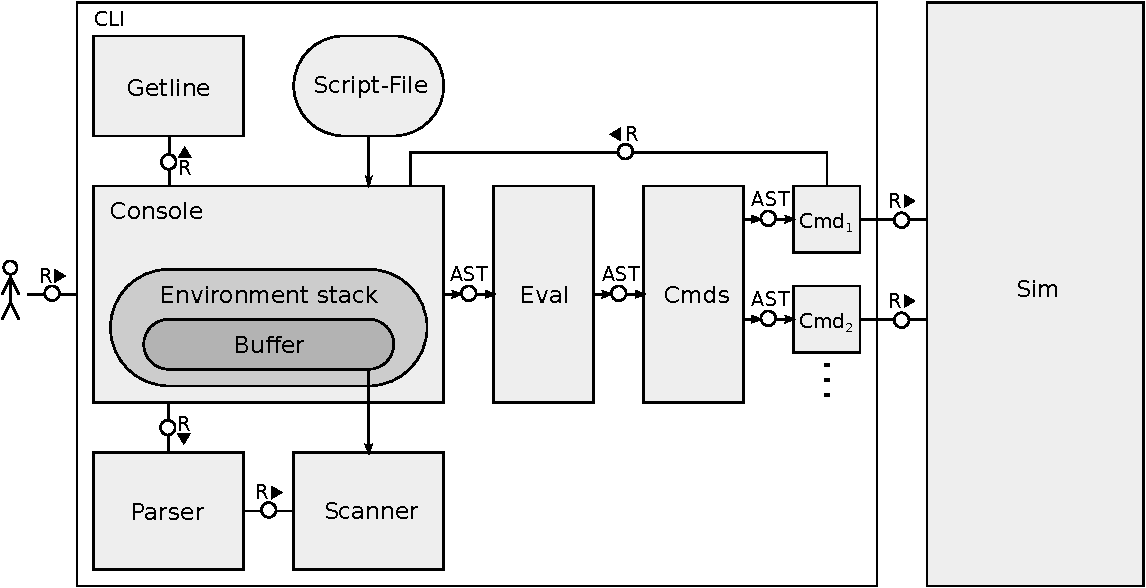
\includegraphics[width=\textwidth]{img/cli-fmc-crop.pdf}
	\caption{Architecture of the CLI in \protect\gls{FMC} notation}
\end{figure}
\noindent Conceptually, the user interacts with the CLI, whose main module is the \i{console}. Depending on whether the console is used interactively or not, it either uses the \i{getline} library\footnote{A small library, that allows basic line editing and provides a history, written by Chris Thewalt. It can be found in the folder \file{lib/getline} of GIMMIX.}  to read a line from the command line into the buffer or reads a specified script file into the buffer. Afterwards this input is parsed to construct an abstract syntax tree (\gls{AST}). The scanner and parser for this task have been generated by \gls{flex} and \gls{Bison}, respectively. As soon as the \gls{AST} is present, it is passed to the \i{eval} module, which executes it. If a node that represents a command is found, the module \i{cmds} comes into play. It holds a table with all available commands and will execute the corresponding function to execute the command. The commands will typically control the simulator, read the state or manipulate it.

As the FMC diagram indicates, the console manages a stack of \i{environments} to allow nesting. Each line or script execution will get a new environment on the top of the stack. This way, a command may use the console to execute a line or script as well. For example, the command \gcmd{tr} uses this feature by storing the desired command as a string and executing it later with the console.

\subsubsection{Command Infrastructure}

Because it is expected that the CLI language itself will not change much in future, but the commands will probably be changed and -- most important -- new ones will be added, it has been decided to separate cleanly between the language and the commands. Additionally, implementing and adding new commands should be as simple as possible. Similarly to the device infrastructure of GIMMIX, a compromise between dynamic and simplicity has been selected. That is, the module cmds keeps a table with all commands, but each command is implemented in its own file. Thus, to add a new command, a file has to be added and the table has to be extended.

Each command has an \i{execution function}, which receives the number of arguments and an array of \gls{AST} nodes -- one for each argument. Additionally, the cmds module provides the function `cmds_evalArg`:
\begin{lstlisting}[language=GIMMIXC]
sCmdArg cmds_evalArg(const sASTNode *arg,int expTypes,octa offset,bool *finished);
\end{lstlisting}
The function receives the argument to evaluate, the types that are supported (integer, float or string), an offset and a pointer to a boolean. The last two are used to implement ranges. Since the language is intended for scripting as well and it is imaginable that a user would like to, \eg, execute 1000 instructions and pipe the contents of the first 64 megabytes of memory into a file to analyze it with other tools later, it has been decided not to simply convert a range to an array. Because as the example shows, it might cost a lot of time and memory. Instead, the evaluation function receives the current offset and tells the caller whether all ranges are already finished. That means, in each step one value of each range is extracted, depending on the current offset.

The return value of `cmds_evalArg` is a struct called `sCmdArg`, that provides all required information about the value of the argument for the caller. It contains the type (integer, float or string), the origin (\gcmd{M8}, \gcmd{l}, \gcmd{\$}, and so on or an arbitrary expression such as \gcmd{1+2}), the location for origins like virtual memory or registers (that is, the memory address or register index) and of course the value of the argument as integer, float or string. The location and origin are for example used by \gcmd{p} to print the origin of an argument or by \gcmd{set} to set the corresponding entity of GIMMIX.

\subsubsection{Command Implementation}

A typical command, that makes use of ranges, is \i{disassemble}. Ignoring the details of the disassembling process, its implementation looks like the following:
\begin{lstlisting}[language=GIMMIXC,caption={Implementation of command \gcmd{d}}]
void cli_cmd_disasm(size_t argc,const sASTNode **argv) {
	if(argc > 1)
		cmds_throwEx(NULL);
	if(argc == 0) {
		for(int i = 0; i < DEFAULT_INSTR_COUNT; i++)
			doDisasm(cpu_getPC() + i * sizeof(tetra));
	}
	else {
		sCmdArg a;
		bool fin = false;
		for(octa off = 0; ; off += sizeof(tetra)) {
			a = cmds_evalArg(argv[0],ARGVAL_INT,off,&fin);
			if(fin)
				break;
			doDisasm(a.d.integer & -(octa)sizeof(tetra));
		}
	}
}
\end{lstlisting}
As the listing shows, at first the number of arguments is checked and if no arguments are given, `DEFAULT_INSTR_COUNT` (16) instructions at the PC will be disassembled. If one argument is given, `cmds_evalArg` will be called until `fin` has been set to `true`, whereas in each step the offset `off` will be increased to reach the next instruction. Thus, "\gcmd{d @:16}" would disassemble the instructions at addresses `@`, `@+4`, `@+8` and `@+12`.

Another interesting example, that utilizes the origin and location, is the command \gcmd{set}. The slightly shortened implementation is:
\begin{lstlisting}[language=GIMMIXC,caption={Implementation of command \gcmd{set}}]
void cli_cmd_set(size_t argc,const sASTNode **argv) {
	if(argc != 2)
		cmds_throwEx(NULL);
	for(octa off = 0; ; off++) {
		bool oFin = false, vFin = false;
		sCmdArg obj,val;
		obj = cmds_evalArg(argv[0],ARGVAL_INT,off,&oFin);
		val = cmds_evalArg(argv[1],
			ARGVAL_INT | ARGVAL_FLOAT,off,&vFin);
		if(oFin)
			break;

		switch(obj.origin) {
			case ORG_VMEM1:
				mmu_writeByte(obj.location,val.d.integer,0);
				break;
			...
			case ORG_EXPR:
				cmds_throwEx("Can't set arbitrary expr\n");
				break;
		}
	}
}
\end{lstlisting}
That means, it iterates over both the objects to set and the values at the same time, until the last object has been assigned. Additionally, the origin is used to determine what entity of GIMMIX should be changed. Of course, \gcmd{set} is not possible for expressions like \gcmd{1*2+M[0]} as first argument. It is only allowed for the \glslink{PC}{instruction pointer} and for fetches, that are specified without any operator in the "outmost layer", \ie \gcmd{M4[@+4]} for example.


